\documentclass{article}

\usepackage{caption}

\usepackage{xcolor}

\usepackage{graphicx}

\usepackage{hyperref}

\usepackage[backend=biber,style=apa]{biblatex}



\addbibresource{bibliography.bib}

\begin{filecontents}[bibliography.bib]
	@article{bib0,
    author      = {undefined, A.U.T.H.O.R.},
    date        = {2020}
}


@article{bib1,
    author      = {undefined, A.U.T.H.O.R.},
    date        = {2014}
}


@article{CSL_BIBLIOGRAPHYAnderson2019,
    title       = {On the automaticity of attentional orienting to threatening stimuli},
    author      = {CSL_BIBLIOGRAPHYAnderson, A.D.D.I.N.ZOTERO_BIBL {"uncited",],"omitted",],"custom",]} and A., B. and Britton, M.K.},
    url         = {https://doi.org/10.1037/emo0000596},
    doi         = {10.1037/emo0000596},
    date        = {2019}
}


@article{Becker2017,
    title       = {The capture of attention and gaze in the search for emotional photographic faces},
    author      = {Becker, S.I. and Dutt, N. and Vromen, J.M.G. and Horstmann, G.},
    number      = {1–3},
    volume      = {25},
    url         = {https://doi.org/10.1080/13506285.2017.1333182},
    doi         = {10.1080/13506285.2017.1333182},
    date        = {2017},
    pages       = {241–261},
    journal     = {Visual Cognition}
}


@article{Cane2009,
    title       = {The addiction Stroop task: Examining the fast and slow effects of smoking and marijuana-related cues},
    author      = {Cane, J. and Sharma, D. and Albery, I.},
    number      = {5},
    volume      = {23},
    url         = {https://doi.org/10.1177/0269881108091253},
    doi         = {10.1177/0269881108091253},
    date        = {2009},
    pages       = {510–519},
    journal     = {Journal of Psychopharmacology}
}


@article{Carlson2020,
    title       = {The stability and reliability of attentional bias measures in the dot-probe task: Evidence from both traditional mean bias scores and trial-level bias scores},
    author      = {Carlson, J.M. and Fang, L.},
    volume      = {13},
    date        = {2020},
    journal     = {Motivation and Emotion}
}


@article{Carlson2014,
    title       = {Attending to the fear in your eyes: Facilitated orienting and delayed disengagement},
    author      = {Carlson, J.M. and Reinke, K.S.},
    number      = {8},
    volume      = {28},
    url         = {https://doi.org/10.1080/02699931.2014.885410},
    doi         = {10.1080/02699931.2014.885410},
    date        = {2014},
    pages       = {1398–1406},
    journal     = {Cognition and Emotion}
}


@article{Carretié2014,
    title       = {Exogenous (automatic) attention to emotional stimuli: A review},
    author      = {Carretié, L.},
    number      = {4},
    volume      = {14},
    url         = {https://doi.org/10.3758/s13415-014-0270-2},
    doi         = {10.3758/s13415-014-0270-2},
    date        = {2014},
    pages       = {1228–1258},
    journal     = {Cognitive, Affective, & Behavioral Neuroscience}
}


@article{Clarke2015,
    title       = {Examining fast and slow effects for alcohol and negative emotion in problem and social drinkers},
    author      = {Clarke, S.P. and Sharma, D. and Salter, D.},
    number      = {1},
    volume      = {23},
    url         = {https://doi.org/10.3109/16066359.2014.922961},
    doi         = {10.3109/16066359.2014.922961},
    date        = {2015},
    pages       = {24–33},
    journal     = {Addiction Research & Theory}
}


@article{Desimone1995,
    title       = {Neural Mechanisms of Selective Visual Attention},
    author      = {Desimone, R. and Duncan, J.},
    date        = {1995}
}


@article{Duthoo2014,
    title       = {The heterogeneous world of congruency sequence effects: An update},
    author      = {Duthoo, W. and Abrahamse, E.L. and Braem, S. and Boehler, C.N. and Notebaert, W.},
    volume      = {5},
    url         = {https://doi.org/10.3389/fpsyg.2014.01001},
    doi         = {10.3389/fpsyg.2014.01001},
    date        = {2014},
    journal     = {Frontiers in Psychology}
}


@article{Fox2001,
    title       = {Do threatening stimuli draw or hold visual attention in subclinical anxiety?},
    author      = {Fox, E. and Russo, R. and Bowles, R. and Dutton, K.},
    number      = {4},
    volume      = {130},
    url         = {https://doi.org/10.1037/0096-3445.130.4.681},
    doi         = {10.1037/0096-3445.130.4.681},
    date        = {2001},
    pages       = {681–700},
    journal     = {Journal of Experimental Psychology: General}
}


@article{Gladwin2017,
    title       = {Carryover effects in spatial attentional bias tasks and their relationship to subclinical PTSD symptoms},
    author      = {Gladwin, T.E.},
    number      = {4},
    volume      = {23},
    url         = {https://doi.org/10.1037/trm0000121},
    doi         = {10.1037/trm0000121},
    date        = {2017},
    pages       = {303},
    journal     = {Traumatology}
}


@article{Gladwin2017,
    title       = {Carryover effects in spatial attentional bias tasks and their relationship to subclinical PTSD symptoms},
    author      = {Gladwin, T.E.},
    number      = {4},
    volume      = {23},
    url         = {https://doi.org/10.1037/trm0000121},
    doi         = {10.1037/trm0000121},
    date        = {2017},
    pages       = {303–308},
    journal     = {Traumatology}
}


@article{Gladwin2019,
    title       = {Trial-to-trial carryover effects on spatial attentional bias},
    author      = {Gladwin, T.E. and Figner, B.},
    volume      = {196},
    url         = {https://doi.org/10.1016/j.actpsy.2019.04.006},
    doi         = {10.1016/j.actpsy.2019.04.006},
    date        = {2019},
    pages       = {51–55},
    journal     = {Acta Psychologica}
}


@article{Gladwin2019,
    title       = {Anticipation-specific reliability and trial-to-trial carryover of anticipatory attentional bias for threat},
    author      = {Gladwin, T.E. and Figner, B. and Vink, M.},
    number      = {7},
    volume      = {31},
    url         = {https://doi.org/10.1080/20445911.2019.1659801},
    doi         = {10.1080/20445911.2019.1659801},
    date        = {2019},
    pages       = {750–759},
    journal     = {Journal of Cognitive Psychology}
}


@article{Gladwin2020,
    title       = {Attentional bias for negative expressions depends on previous target location: Replicable effect but unreliable measures},
    author      = {Gladwin, T.E. and Jewiss, M. and Vink, M.},
    url         = {https://doi.org/10.1080/20445911.2020.1805453},
    doi         = {10.1080/20445911.2020.1805453},
    date        = {2020},
    pages       = {1–11},
    journal     = {Journal of Cognitive Psychology}
}


@article{Gur2002,
    title       = {A method for obtaining 3-dimensional facial expressions and its standardization for use in neurocognitive studies},
    author      = {Gur, R.C. and Sara, R. and Hagendoorn, M. and Marom, O. and Hughett, P. and Macy, L. and Turner, T. and Bajcsy, R. and Posner, A. and Gur, R.E.},
    number      = {2},
    volume      = {115},
    url         = {https://doi.org/10.1016/S0165-0270(02)00006-7},
    doi         = {10.1016/S0165-0270(02)00006-7},
    date        = {2002},
    pages       = {137–143},
    journal     = {Journal of Neuroscience Methods}
}


@article{Hedge2018,
    title       = {The reliability paradox: Why robust cognitive tasks do not produce reliable individual differences},
    author      = {Hedge, C. and Powell, G. and Sumner, P.},
    number      = {3},
    volume      = {50},
    url         = {https://doi.org/10.3758/s13428-017-0935-1},
    doi         = {10.3758/s13428-017-0935-1},
    date        = {2018},
    pages       = {1166–1186},
    journal     = {Behavior Research Methods}
}


@article{Hedger2016,
    title       = {Are visual threats prioritized without awareness? A critical review and meta-analysis involving 3 behavioral paradigms and 2696 observers},
    author      = {Hedger, N. and Gray, K.L.H. and Garner, M. and Adams, W.J.},
    number      = {9},
    volume      = {142},
    url         = {https://doi.org/10.1037/bul0000054},
    doi         = {10.1037/bul0000054},
    date        = {2016},
    pages       = {934–968},
    journal     = {Psychological Bulletin}
}


@article{Hill2016,
    title       = {Exploring Carry-Over Effects to Elucidate Attention Bias Modification’s Mixed Results},
    author      = {Hill, M. and Duval, E.},
    url         = {https://doi.org/10.22186/jyi.31.3.9-14},
    doi         = {10.22186/jyi.31.3.9-14},
    date        = {2016},
    journal     = {Journal of Young Investigators}
}


@article{Ho2019,
    title       = {Moving beyond P values: Data analysis with estimation graphics},
    author      = {Ho, J. and Tumkaya, T. and Aryal, S. and Choi, H. and Claridge-Chang, A.},
    number      = {7},
    volume      = {16},
    url         = {https://doi.org/10.1038/s41592-019-0470-3},
    doi         = {10.1038/s41592-019-0470-3},
    date        = {2019},
    pages       = {565–566},
    journal     = {Nature Methods}
}


@article{Imhoff2019,
    title       = {Identification and location tasks rely on different mental processes: A diffusion model account of validity effects in spatial cueing paradigms with emotional stimuli},
    author      = {Imhoff, R. and Lange, J. and Germar, M.},
    number      = {2},
    volume      = {33},
    url         = {https://doi.org/10.1080/02699931.2018.1443433},
    doi         = {10.1080/02699931.2018.1443433},
    date        = {2019},
    pages       = {231–244},
    journal     = {Cognition and Emotion}
}


@article{Kruijt2016,
    title       = {Capturing Dynamics of Biased Attention: Are New Attention Variability Measures the Way Forward?},
    author      = {Kruijt, A.-W. and Field, A.P. and Fox, E.},
    number      = {11},
    volume      = {11},
    url         = {https://doi.org/10.1371/journal.pone.0166600},
    doi         = {10.1371/journal.pone.0166600},
    date        = {2016},
    pages       = {0166600},
    journal     = {PLOS ONE}
}


@article{Kruijt2018,
    title       = {A Meta-Analysis of Bias at Baseline in RCTs of Attention Bias Modification: No Evidence for Dot-Probe Bias Towards Threat in Clinical Anxiety and PTSD},
    author      = {Kruijt, A.-W. and Parsons, S. and Fox, E.},
    volume      = {11},
    date        = {2018},
    journal     = {Journal of Abnormal Psychology}
}


@report{Lang2008,
    title       = {International affective picture system (IAPS): Affective ratings of pictures and instruction manual},
    author      = {Lang, P.},
    url         = {https://ci.nii.ac.jp/naid/20001061266/},
    date        = {2008}
}


@book{Lundqvist1998,
    title       = {The Karolinska Directed Emotional Faces (KDEF},
    author      = {Lundqvist, Flykt and A. and Ohman, A.},
    publisher   = {Department of Neurosciences Karolinska Hospital},
    place       = {Stockholm},
    date        = {1998}
}


@article{MacLeod1986,
    title       = {Attentional bias in emotional disorders},
    author      = {MacLeod, C. and Mathews, A. and Tata, P.},
    number      = {1},
    volume      = {95},
    url         = {https://doi.org/10.1037/0021-843X.95.1.15},
    doi         = {10.1037/0021-843X.95.1.15},
    date        = {1986},
    pages       = {15–20},
    journal     = {Journal of Abnormal Psychology}
}


@article{Mogg1998,
    title       = {A cognitive-motivational analysis of anxiety},
    author      = {Mogg, K. and Bradley, B.P.},
    number      = {9},
    volume      = {36},
    url         = {https://doi.org/10.1016/S0005-7967(98)00063-1},
    doi         = {10.1016/S0005-7967(98)00063-1},
    date        = {1998},
    pages       = {809–848},
    journal     = {Behaviour Research and Therapy}
}


@article{Mogg2017,
    title       = {Attention Bias Modification (ABM): Review of Effects of Multisession ABM Training on Anxiety and Threat-Related Attention in High-Anxious Individuals},
    author      = {Mogg, K. and Waters, A.M. and Bradley, B.P.},
    number      = {4},
    volume      = {5},
    url         = {https://doi.org/10.1177/2167702617696359},
    doi         = {10.1177/2167702617696359},
    date        = {2017},
    pages       = {698–717},
    journal     = {Clinical Psychological Science}
}


@article{Panksepp2011,
    title       = {What is Basic about Basic Emotions? Lasting Lessons from Affective Neuroscience},
    author      = {Panksepp, J. and Watt, D.},
    number      = {4},
    volume      = {3},
    url         = {https://doi.org/10.1177/1754073911410741},
    doi         = {10.1177/1754073911410741},
    date        = {2011},
    pages       = {387–396},
    journal     = {Emotion Review}
}


@article{Posner1985,
    title       = {Inhibition of return: Neural basis and function},
    author      = {Posner, M.I. and Rafal, R.D. and Choate, L.S. and Vaughan, J.},
    number      = {3},
    volume      = {2},
    url         = {https://doi.org/10.1080/02643298508252866},
    doi         = {10.1080/02643298508252866},
    date        = {1985},
    pages       = {211–228},
    journal     = {Cognitive Neuropsychology}
}


@article{Schmukle2005,
    title       = {Unreliability of the dot probe task},
    author      = {Schmukle, S.C.},
    number      = {7},
    volume      = {19},
    url         = {https://doi.org/10.1002/per.554},
    doi         = {10.1002/per.554},
    date        = {2005},
    pages       = {595–605},
    journal     = {European Journal of Personality}
}


@article{Schubö2006,
    title       = {Detecting emotional faces and features in a visual search paradigm: Are faces special?},
    author      = {Schubö, A. and Gendolla, G.H.E. and Meinecke, C. and Abele, A.E.},
    number      = {2},
    volume      = {6},
    url         = {https://doi.org/10.1037/1528-3542.6.2.246},
    doi         = {10.1037/1528-3542.6.2.246},
    date        = {2006},
    pages       = {246–256},
    journal     = {Emotion}
}


@article{Staugaard2009,
    title       = {Reliability of two versions of the dot-probe task using photographic faces},
    author      = {Staugaard, S.R.},
    number      = {3},
    volume      = {51},
    date        = {2009},
    pages       = {339–350},
    journal     = {Psychological Science Quarterly}
}


@article{Waters2005,
    title       = {Generalizability of carry-over effects in the emotional Stroop task},
    author      = {Waters, A.J. and Sayette, M.A. and Franken, I.H.A. and Schwartz, J.E.},
    number      = {6},
    volume      = {43},
    url         = {https://doi.org/10.1016/j.brat.2004.06.003},
    doi         = {10.1016/j.brat.2004.06.003},
    date        = {2005},
    pages       = {715–732},
    journal     = {Behaviour Research and Therapy}
}


@article{Wilson2007,
    title       = {Carry-over effects of smoking cue exposure on working memory performance},
    author      = {Wilson, S.J. and Sayette, M.A. and Fiez, J.A. and Brough, E.},
    number      = {5},
    volume      = {9},
    url         = {https://doi.org/10.1080/14622200701243144},
    doi         = {10.1080/14622200701243144},
    date        = {2007},
    pages       = {613–619},
    journal     = {Nicotine & Tobacco Research}
}


@article{Zvielli2015,
    title       = {Temporal Dynamics of Attentional Bias},
    author      = {Zvielli, A. and Bernstein, A. and Koster, E.H.W.},
    number      = {5},
    volume      = {3},
    url         = {https://doi.org/10.1177/2167702614551572},
    doi         = {10.1177/2167702614551572},
    date        = {2015},
    pages       = {772–788},
    journal     = {Clinical Psychological Science}
}
\end{filecontents}

\begin{document}


	Title



	Carryover Effects for Threat in the Dot-Probe Task







	Abstract



	Threatening stimuli are often thought to have sufficient potency to bias attention, relative to neutral stimuli. Researchers and clinicians opt for frequently used paradigms to measure such bias, such as the dot-probe task. Bias to threat in the dot-probe task is indicated by a congruency effect i.e., faster responses on congruent trials than incongruent trials (also referred to as attention capture). However, recent studies have found that such congruency effects are small and suffer from poor internal reliability. One explanation to low effect sizes and poor reliability is \emph{carryover effects} of threat – greater congruency effects on trials following a congruent trial relative to trials following an incongruent trial. In the current study, we investigated carryover effects of threat with two large samples of healthy undergraduate students who completed a typical dot-probe task. Although we found a small congruency effect for fearful faces (Experiment 1, \emph{n} = 241, \emph{d }= 0.15) and a reverse congruency effect for threatening images, (Experiment 2, \emph{n }= 82, \emph{d }= 0.11) whereas no carryover effects for threat were observed in either case. Bayesian analyses revealed moderate to strong evidence in favor of the null hypothesis. We conclude that carryover effects for threat do not influence attention bias for threat.







	\textbf{Keywords:} dot-probe, emotional cues, carryover effects, attention bias, threat















	Take-home message



	How is attentional bias to threat influenced by recent events? In the current study, we tested whether bias to threat (in the dot-probe task) is greater when threat cues recently appeared in a target location, relative to when they appeared in a non-target location (otherwise known as a carryover effect for threat). While we did not find carryover effects for threat, we suspect they are possible in other paradigms and that they exist in real-life scenarios. Carryover effects for threat in the dot-probe task are not likely to influence congruency effects.







	Purpose



	The objective of this study was to assess whether carryover effects for threat would be observed in the dot-probe task. Related studies have found support for carryover effects for threat \autocite{Gladwin2017}\autocite{Gladwin2017}\autocite{Gladwin2019}\autocite{Gladwin2020}\autocite{Gladwin2019a}. However, there are several unique elements to the task design and procedure used in these studies that make them difficult to compare to the commonly used dot-probe task (a task often used in applied, clinical, and basic research on emotion processing). Our purpose was to extend these previous studies of carryover effects for threat to the standard dot-probe task.























	Do Carryover Effects Influence Attentional Bias to Threat in the Dot-Probe Task?



	Emotional stimuli are thought to receive prioritized processing. Threatening stimuli like angry and fearful facial expressions of emotion often “beat-out” neutral or innocuous objects \autocite{Becker2017}\autocite{Schubö2006} in the competition over spatial attentional resources \autocite{Desimone1995}. Attentional bias to threat is a topic of research that intersects many domains and is an essential function for a variety of organisms \autocite{Anderson2019}.



	One of the most commonly used tasks to assess attentional bias to threat is the dot-probe task \autocite{MacLeod1986}. In a typical dot-probe task, participants search for the location of a target dot and indicate its position (left or right side of the screen) with a corresponding keypress. Immediately prior to the presentation of the target dot, two adjacent cues (one neutral and one threatening cue) are simultaneously presented for a very brief period (e.g., 100 millisecond (ms)). On congruent trials, the dot appears at the location of the threatening cue, whereas on incongruent trials, the dot appears at the location of the neutral cue (see Figure 1A). Each cue is completely irrelevant to the current task demands. And yet, the threatening cue biases attention to a greater extent than the neutral cue, as shown by faster response times (RTs) for congruent trials relative to incongruent trials (for reviews, see \autocite{Carretié2014}\autocite{Imhoff2019}. This effect is known as a \emph{congruency effect}, or attentional capture by threat or attentional bias to threat.



	While congruency effects are often assessed by the dot-probe task \autocite{Kruijt2018}\autocite{Mogg2017}, they have come under scrutiny for poor internal and test-retest reliability \autocite{Schmukle2005}\autocite{Staugaard2009}. One root cause of these issues is that difference scores are inherently unreliable \autocite{Hedge2018}. However, some studies have found that attention (and congruency effects) may fluctuate towards and away from threat during the course of an experiment (\autocite{Zvielli2015}. This suggests attention bias variability could be a meaningful element of attention bias. However, these trial-to-trial variability measures appear to be strongly related to general RT variability (\autocite{Carlson2020}\autocite{Kruijt2016}. Identifying new sources of potential variation—like carryover effects —in the dot-probe task is beneficial because they could be accounted for in future studies.



	Carryover Effects



	Suppose that an individual’s attention was biased towards a threatening stimulus—like a fearful face—during a congruent trial of a dot-probe task. Such bias could impact the individual’s internal state \autocite{Panksepp2011}, priming, or increase their association between the target and the threatening cue, which could subsequently cause them to be more biased towards threat in later trials. A persistent bias for threatening stimuli is quite plausible given that threatening cues can also bring about attentional dwelling towards themselves \autocite{Carlson2014}\autocite{Fox2001}. In the past, others have found carryover effects in the emotional Stroop \autocite{Cane2009}\autocite{Clarke2015}\autocite{Waters2005}\autocite{Wilson2007} and diagonalized visual probe task \autocite{Gladwin2019}\autocite{Gladwin2020}\autocite{Gladwin2019a}. In these tasks, attentional bias to an emotional cue (i.e., difference in RTs between congruent and incongruent trials) is greater when the previous trial is congruent, otherwise known as a \emph{carryover effect }\autocite{Gladwin2019}.



	As for dot-probe studies, however, there is not yet a clear answer on this topic given the very limited number of studies. In one dot-probe study that used threatening faces, no carryover effects were observed \autocite{Hill2016}. In another study, carryover effects were only observed for accuracy measures, and not RTs (for non-face stimuli, \autocite{Gladwin2017}. But these two studies have serious limitations: one used a small sample \autocite{Gladwin2017}, and the other measured carryover effects after attention training was administered \autocite{Hill2016}. Here we improve upon these limitations by examining the same question with a large sample of healthy undergraduate students who completed a typical dot-probe task.



	The Current Study



	In the current study, we sought to test carryover effects for threat in the dot-probe task. To test this question, we performed a secondary data analysis on two dot-probe experiments with fearful facial stimuli (Experiment 1) and threatening pictorial stimuli (Experiment 2; AUTHOR, 2020). We consider fearful faces and pictorial images of threat to be threatening because a recent meta-analysis on threat detection examined both of them \autocite{Hedger2016}. Based on previous research \autocite{Gladwin2019a}\autocite{Gladwin2020a}, we hypothesized that there would be such an influence (as indicated by an interaction between previous trial congruency and current trial congruency). More specifically, we expected that current trial congruency effects would be larger when the previous trial was congruent, relative to when it was incongruent (see Figure 1B). If our hypothesis was confirmed, we would have identified an important source of variability in the dot-probe task. On the other hand, if our hypothesis was not supported, we would conclude that the influence of carryover effects on congruency effects is negligible.



	Experiment 1



	\subsubsection{Methods}



	\emph{Participants. }Participants with an overall accuracy below 90% percent (eight in total) were removed from all analyses, leaving a final sample size of 241 (\emph{M}\textsubscript{\emph{age}} = 21.4, \emph{SD}\textsubscript{\emph{age}} = 4.3; 178 females). The data reported here were acquired during a screening session of a larger study on attention bias modification and brain structure, funded by the National Institute of Mental Health (NCT03092609). A portion of the current sample (\emph{n} = 127) were included in Experiment 1 of \autocite{Carlson2020}. The study was approved by the UNIVERSITY Institutional Review Board. Participants received monetary compensation for their participation.



	\emph{Stimuli and Apparatus. }The procedure was administered with a PC and a 16” LCD computer monitor. Stimuli consisted of 20 fearful and neutral grayscale faces of 10 different actors (half female; \autocite{Gur2002}\autocite{Lundqvist1998}. Fearful faces were rated (1-9, unpleasant to pleasant) as more negative (\emph{M} = 3.83, \emph{SD} = 0.30) than neutral pictures (\emph{M} = 4.45, \emph{SD} = 0.52), \emph{t}(18) = 3.23, \emph{p} = .005, \emph{d} = 1.48. Faces subtended a visual width and height of 5 × 7 and the distance between the center of each face subtended 14.



	\textbf{[Insert Figure 1 here]}



	\emph{Design. }The experiment consisted of five blocks of trials and each block consisted of 90 trials for a total of 450 trials. 30 congruent, 30 incongruent, and 30 baseline trials were randomly presented within each block. During baseline trials, two neutral faces were shown in the cue display and the dot was randomly presented in the same position as one of the two neutral faces (one third of all trials). Baseline trials were not included in our analyses. See Figure 1A for examples of incongruent and congruent trials.



	\emph{Procedure. }Each trial started with a white fixation cross (+) in the center of a black screen for 1000 ms, which was immediately followed by the cue display. The cue display was presented for 100 ms. In the cue display, there were two bilaterally presented faces. Immediately following the cue display, a single dot (the target object) was randomly presented in the central position of one of the previously shown faces in the cue display until participants responded. Participants indicated the location of the dot (left or right side of the display) by pressing a corresponding button with the pointer or middle finger of their right hand.



	Results



	All trials with an incorrect response (2.2% of trials) or a response time outside of 3 standard deviations from the individual-wise and condition means were removed from all RT analyses (0.6% of trials). Attentional bias was measured by subtracting mean RTs for congruent trials from incongruent trials. Positive values indicate the level of attentional bias for fearful faces. All analyses were not pre-registered but were pre-planned. As shown in Figure 2A, RTs for congruent trials (\emph{M = }331 ms, \emph{SD} of 72 ms) were significantly shorter for incongruent trials (\emph{M = }342 ms, \emph{SD} of 72 ms), \emph{t}(240) = 20.56, \emph{p} < .001, \emph{d }= 0.16. A congruency effect was also found for percent correct (1.5%), \emph{t}(240) = 14.31, \emph{p} < .001, \emph{d }= 0.11.



	As shown in Figure 2B, carryover effects are measured as the interaction between previous trial congruency (pre-congruent or pre-incongruent) and current trial congruency (congruent or incongruent). The location of the fearful face and the target could repeat from trial to trial, so we further separated carryover effects by target location repetition. We examined target location repetition for two reasons: (a) it is an exploratory approach to analyzing carryover effects and (b) previous studies on carryover effects \autocite{Gladwin2019a} have deliberately prevented cue and target locations repetitions trial-to-trial. We tested for the presence of carryover effects by conducting a 2 × 2 × 2 Generalized Linear Mixed Model (GLMM) with the random effect of subject and the fixed effects of current trial congruency (congruent or incongruent), previous trial congruency (pre-congruent or pre-incongruent) and target location repetition (repeated or non-repeated) on single trial RTs using a Gamma probability distribution with a log link, which accounts for the slightly positive skew of the data\footnote{{\color{ }}{\color{We also tested a model with a random slope for congruency x previous congruency x target location repetition interaction. Although }}{\color{this}}{\color{ model fit our data better (AIC}}\textsubscript{{\color{without random slope}}}{\color{ = -26903.474 whereas AIC}}\textsubscript{{\color{with random slope}}}{\color{ = -27133.846}}{\color{;}}{\color{models with smaller AIC values fit better), the significant levels of all the fixed effect}}{\color{s}}{\color{ for this model was very similar to the one reported in the main text, where there was no significant carryover effect.}}}. Target location repetition was included in the model because previous studies of carryover effects deliberately chose to prevent target locations repetition between trials \autocite{Gladwin2019a}, which leaves open the possibility that target repetition may moderate carryover effects. Similar to the t-test reported above, there was a main effect of current trial type, \emph{F}(1, 46115) = 348.91, \emph{p }< .001: RTs were faster on congruent (\emph{M }= 329, \emph{SD}\emph{ }= 68) relative to incongruent (\emph{M }= 339, \emph{SD }= 69) trials. There was also a main effect of target location repetition (\emph{F}(1, 46115) = 222.06, \emph{p }< .001) wherein RTs were faster for non-repeated target locations (\emph{M }= 330, \emph{SE }= 2.32) relative to repeated locations (\emph{M }= 338, \emph{SE }= 2.38). There was also an interaction between target location repetition and previous trial congruency (\emph{F}(1, 46115) = 6.08, \emph{p }= .01) such that RTs for non-repeated target locations were faster if the previous trial was congruent (\emph{M }= 329, \emph{SE }= 2.34) relative to incongruent (\emph{M }= 331, \emph{SE }= 2.36). Meanwhile, for repeated target location there was no statistically significant difference in RTs between trials where the previous trial was congruent (\emph{M }= 339, \emph{SE }= 2.42) relative to incongruent (\emph{M }= 338, \emph{SE }= 2.42). Critically, neither the 2-way interaction between current trial congruency and previous trial congruency (\emph{F}(1, 46115) = 0.59, \emph{p }= .44) nor the 3-way interaction (\emph{F}(1, 46115) = 0.84, \emph{p }= .36) were significant, indicating that no carryover effects were observed. No other effects were significant.



	We followed up the GLMM approach with a Bayesian analysis. Given that there were no clear prior probabilities based on previous research, a diffuse (or uninformative) prior was used in SPSS to quantify evidence for the null hypothesis that there is no carryover effect for threat. A Bayes Factor analysis on a related-sample t-test indicated moderate evidence for the null hypothesis (BF01 = 5.38). In other words, the data is 5.38 times as likely under the null hypothesis than under the alternative hypothesis (i.e., that there is an influence of previous trial congruency on current trial congruency).



	Experiment 2



	In Experiment 2, our goal was to replicate and extend our lack of carryover effects with another category of threatening stimuli: threatening images \autocite{Lang2008}. We used data from Experiment 2 of \autocite{Carlson2020}. The method for Experiment 2 is the same as Experiment 1 except for the following.



	\subsubsection{Method}



	\emph{Participants. }Participants with an overall accuracy below 90% percent (4 in total) were removed from all analyses, leaving a final sample size of 82 (\emph{M}\textsubscript{\emph{age}} = 20, \emph{SD}\textsubscript{\emph{age}} = 2.2; 61 females).



	\emph{Stimuli and Apparatus. }The visual angle between the two stimuli presented in the cue display subtended a visual angle of 12°. The images used in the cue display were taken from the International Affective Picture System (IAPS; \autocite{Lang2008}. 10 threatening and 10 neutral images were used, and the cue display was shown for 500 ms.



	\subsubsection{Results}



	\subsection{Outlier RT trials were removed from all analyses (0.5% of trials). To test for carryover effects, we conducted the same 2 × 2 × 2 Generalized Linear Mixed Model on RTs as in Experiment 1. There was a main effect of current trial type (\emph{F}(1, 15869) = 16.21, \emph{p }< .001) wherein RTs were faster for incongruent (\emph{M }= 345 , \emph{SE }= 4.06) relative to congruent trials (\emph{M }= 349, \emph{SE }= 4.11). Note that this effect indicates attentional bias to neutral, not threatening images, (see Figure 2C) which also might indicate for threatening images. There was also a main effect of target location repetition, \emph{F}(1, 15869 = 167.53, \emph{p }< .001), wherein RTs were faster for trials with non-repeated target locations (\emph{M }= 340, \emph{SE }= 4.00) compared to repeated locations (\emph{M }= 354, \emph{SE }= 4.17). However, as in Experiment 1, neither the 2-way interaction between current trial congruency and previous trial congruency (\emph{F}(1, 15869) = 0.53, \emph{p }= .47) nor were the 3-way interactions (\emph{F}(1, 15869) = 0.01, \emph{p }= .92) significant (see Figure 2D). Thus, no carryover effects were observed. In addition, no other effects were significant. We again followed up the GLMM approach with the same Bayesian analysis. For Experiment 2, we found strong evidence for the null hypothesis (BF01 = 11.27) indicating that the data are 11.27 times more likely under the null hypothesis than under the hypothesized existence of a carryover effect for threat. }



	\subsection{\textbf{[Insert Figure 2 Here]}}



	Discussion



	In two dot-probe experiments, we assessed whether attentional bias to fearful faces (Experiment 1) or threatening images (Experiment 2) would be influenced by carryover effects. Given that threatening stimuli are especially salient, their potential trial-to-trial influence on attention is quite plausible. However, the evidence supporting carryover effects for threat has been insufficient to rule out the influence of carryover effects \autocite{Gladwin2019a}\autocite{Hill2016}. In Experiment 1, while we did observe a small sized congruency effect for fearful faces, we did not find an interaction between current trial congruency and previous trial congruency. Even for non-repeating target location trials (see Figure 1B), we found no such interaction. There are multiple potential explanations for faster responses on non-repeating target location trials. One is that participants strategically attend away from the emotional cue. Another possibility is that participants avoid previous target locations, as explained by inhibition of return \autocite{Posner1985}. Lastly, our non-significant carryover effects for threat were replicated in Experiment 2. The results from our Bayesian analyses showed moderate to strong evidence for this null result.



	The lack of carryover effects we observed is consistent with previous statistical findings from other dot-probe studies \autocite{Gladwin2017}\autocite{Hill2016}\autocite{Hill2016}. These previous studies, when combined with the current findings, strongly suggest that attentional bias for threat in dot-probe tasks (congruent-incongruent) is unlikely to be moderated by carryover effects. Our study improved upon the limitations of these previous studies: we used a very large sample in Experiment 1, and did not administer any prior-experimental manipulations (like attentional training in \autocite{Hill2016}. The current evidence suggests that previous studies and future research involving the dot-probe task do not need to consider whether congruency effects are influenced by carryover effects.



	Carryover effects are analogous to the congruency sequence effect commonly observed in the flanker, Simon, and Stroop tasks \autocite{Duthoo2014}. One difference between the dot-probe task and these other tasks is that the distractor stimulus does not directly conflict with the target. For example, in the Stroop task, the font color of the word stimulus can be incongruent with the meaning of the word, which creates conflict when the goal is to indicate the word color. Similarly, in the arrow flanker task, conflict is created on incongruent trials; the two arrows to the left and two to the right point in the direction opposite to the direction of the center target arrow, like this: < < > < <. On congruent trials, all five of the arrows point in the same direction. However, in the dot-probe task, the target does not co-occur with the conflicting cue (they are shown in different displays); they are separated in time, and they are visually distinct categories of stimuli because the cue is a face, and the target is simply a single dot. Therefore, current trial congruency effects in the dot-probe task may stem from relatively low stimulus conflict and therefore be unaffected by previous trial congruency. In sum, carryover effects, or congruency sequence effects, may only arise for specific types of stimulus conflict.



	There are some notable procedural differences between the standard dot-probe task (as used here) and other studies that used a similar spatial cueing task but did observe carryover effects. For example, in the unique study design by \autocite{Gladwin2019a}\autocite{Gladwin2020a}, they presented their cues until the participants made a response, whereas we only presented our cues for 100 ms (Experiment 1) or 500 ms (Experiment 2). Presenting cues until a response is made increases the possibility of attentional dwelling or delayed disengagement from the cue, as opposed to the initial orienting of attention towards the cue \autocite{Fox2001}. Another key difference is that \autocite{Gladwin2019a}\autocite{Gladwin2020a} presented a distractor (non-target object) in their search display, whereas in the classic dot-probe task, the target appears alone \autocite{Mogg1998}. Inhibition of the cue that appears in the previous non-target location might explain carryover effects for the cue \autocite{Gladwin2020a}. The presence of the non-target distractor might facilitate such inhibition, thereby creating a carryover effect \autocite{Gillich2019}\autocite{Gladwin2019a}. Future studies on carryover effects should carefully consider their task design procedure.



	Conclusion



	Researchers should carefully select their study design when examining congruency effects. As for studies involving the dot-probe task, however, carryover effects for threat do not appear to be a concern. The highly controlled and simple design of the dot-probe task adequately controls for sources of variance such as carryover effects. While threatening cues may bias attention to a greater extent than neutral cues, their residual influence on attention is limited when assessed with the dot-probe task.



	Data Availability Statement:\emph{ }Datasets are available here: https://osf.io/7qhsj/?view_only=07b52294c1b647829644a833fc3d4883







	\begin{figure}
		\caption{}

		\label{fig:rId11}

		
\includegraphics{media/image1.png}
	\end{figure}
	\begin{figure}
		\caption{}

		\label{fig:rId12}

		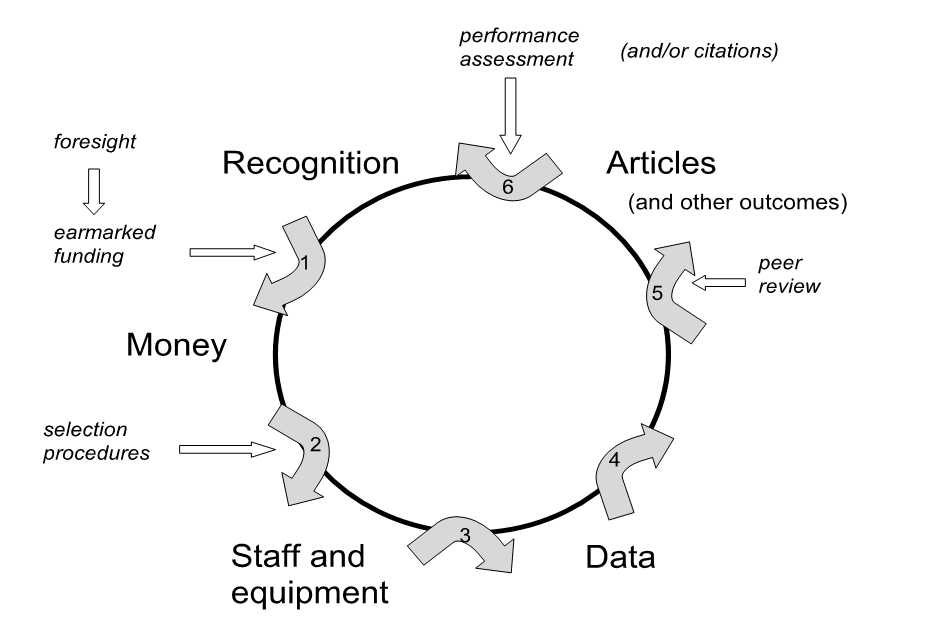
\includegraphics{media/image2.png}
	\end{figure}
	\begin{figure}
		\caption{}

		\label{fig:rId12}

		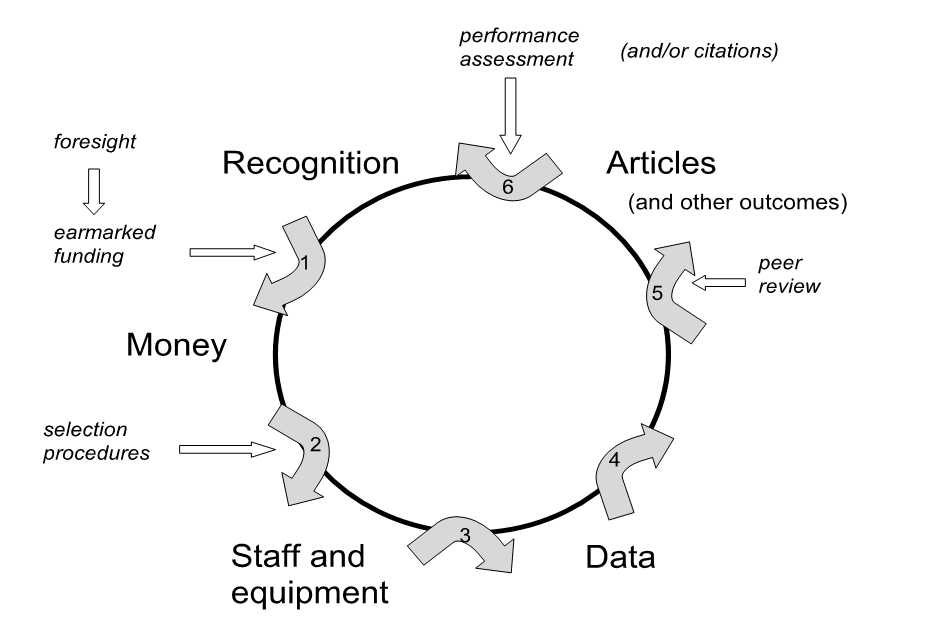
\includegraphics{media/image2.png}
	\end{figure}
	\begin{figure}
		\caption{}

		\label{fig:rId13}

		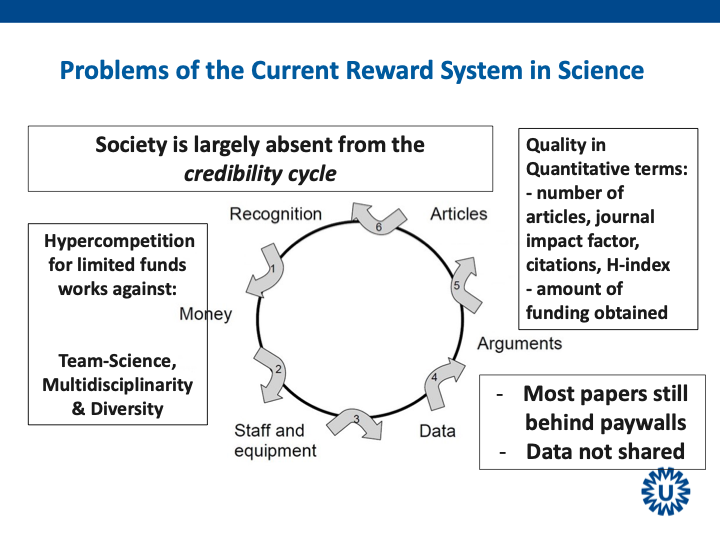
\includegraphics{media/image3.png}
	\end{figure}
	\begin{figure}
		\caption{}

		\label{fig:rId14}

		\includegraphics{media/image4.png}
	\end{figure}



	\emph{Figure 1. }(A) Examples of congruent and incongruent trials in Experiment 1. (B) On the left is an example of two congruent trials—note the target (dot) appears in the location of the fearful face on the previous trial (trial \emph{n-}1) and the current trial (trial \emph{n}). A carryover effect occurs when there is a larger congruency effect when the current congruent trial is preceded by a congruent trial, relative to when it is preceded by an incongruent trial. On the right is an example of two sequential trials where the target appears in the same location (repeating target location).



	\begin{figure}
		\caption{}

		\label{fig:rId15}

		
\includegraphics{media/image5.png}
	\end{figure}



	\emph{Figure 2. }Results from Experiment 1 are shown in A and B, Experiment 2 in C and D (\emph{n} indicates participant, values are averages by participant). A and C show congruent and incongruent RTs (left) and the overall congruency effects (otherwise known as the capturing of attention, or attention bias). The top row of B and D show congruency effects by previous trial congruency and target repetition. The bottom row shows congruency effects by previous trial congruency (incongruent minus congruent), separated by target location repetition. Black error bars represent standard deviation of the mean. Gray distributions represent 95% confidence intervals \autocite{Ho2019}.







	References



	AUTHOR (2020).



	AUTHOR (2014).



	\emph{Emotion}. https://doi.org/10.1037/emo0000596



	Becker, S. I., Dutt, N., Vromen, J. M. G., & Horstmann, G. (2017). The capture of attention and gaze in the search for emotional photographic faces. \emph{Visual Cognition}, \emph{25}(1–3), 241–261. https://doi.org/10.1080/13506285.2017.1333182



	Cane, J., Sharma, D., & Albery, I. (2009). The addiction Stroop task: Examining the fast and slow effects of smoking and marijuana-related cues. \emph{Journal of Psychopharmacology}, \emph{23}(5), 510–519. https://doi.org/10.1177/0269881108091253



	Carlson, J. M., & Fang, L. (2020). The stability and reliability of attentional bias measures in the dot-probe task: Evidence from both traditional mean bias scores and trial-level bias scores. \emph{Motivation and Emotion}, 13.



	Carlson, J. M., & Reinke, K. S. (2014). Attending to the fear in your eyes: Facilitated orienting and delayed disengagement. \emph{Cognition and Emotion}, \emph{28}(8), 1398–1406. psyh. https://doi.org/10.1080/02699931.2014.885410



	Carretié, L. (2014). Exogenous (automatic) attention to emotional stimuli: A review. \emph{Cognitive, Affective, & Behavioral Neuroscience}, \emph{14}(4), 1228–1258. https://doi.org/10.3758/s13415-014-0270-2



	Clarke, S. P., Sharma, D., & Salter, D. (2015). Examining fast and slow effects for alcohol and negative emotion in problem and social drinkers. \emph{Addiction Research & Theory}, \emph{23}(1), 24–33. https://doi.org/10.3109/16066359.2014.922961



	Desimone, R., & Duncan, J. (1995). \emph{Neural Mechanisms of Selective Visual Attention}. 30.



	Duthoo, W., Abrahamse, E. L., Braem, S., Boehler, C. N., & Notebaert, W. (2014). The heterogeneous world of congruency sequence effects: An update. \emph{Frontiers in Psychology}, \emph{5}. https://doi.org/10.3389/fpsyg.2014.01001



	Fox, E., Russo, R., Bowles, R., & Dutton, K. (2001). Do threatening stimuli draw or hold visual attention in subclinical anxiety? \emph{Journal of Experimental Psychology: General}, \emph{130}(4), 681–700. https://doi.org/10.1037/0096-3445.130.4.681



	Gladwin, T. E. (2017a). Carryover effects in spatial attentional bias tasks and their relationship to subclinical PTSD symptoms. \emph{Traumatology}, \emph{23}(4), 303. https://doi.org/10.1037/trm0000121



	Gladwin, T. E. (2017b). Carryover effects in spatial attentional bias tasks and their relationship to subclinical PTSD symptoms. \emph{Traumatology}, \emph{23}(4), 303–308. psyh. https://doi.org/10.1037/trm0000121



	Gladwin, T. E., & Figner, B. (2019). Trial-to-trial carryover effects on spatial attentional bias. \emph{Acta Psychologica}, \emph{196}, 51–55. https://doi.org/10.1016/j.actpsy.2019.04.006



	Gladwin, T. E., Figner, B., & Vink, M. (2019). Anticipation-specific reliability and trial-to-trial carryover of anticipatory attentional bias for threat. \emph{Journal of Cognitive Psychology}, \emph{31}(7), 750–759. https://doi.org/10.1080/20445911.2019.1659801



	Gladwin, T. E., Jewiss, M., & Vink, M. (2020). Attentional bias for negative expressions depends on previous target location: Replicable effect but unreliable measures. \emph{Journal of Cognitive Psychology}, 1–11. https://doi.org/10.1080/20445911.2020.1805453



	Gur, R. C., Sara, R., Hagendoorn, M., Marom, O., Hughett, P., Macy, L., Turner, T., Bajcsy, R., Posner, A., & Gur, R. E. (2002). A method for obtaining 3-dimensional facial expressions and its standardization for use in neurocognitive studies. \emph{Journal of Neuroscience Methods}, \emph{115}(2), 137–143. https://doi.org/10.1016/S0165-0270(02)00006-7



	Hedge, C., Powell, G., & Sumner, P. (2018). The reliability paradox: Why robust cognitive tasks do not produce reliable individual differences. \emph{Behavior Research Methods}, \emph{50}(3), 1166–1186. https://doi.org/10.3758/s13428-017-0935-1



	Hedger, N., Gray, K. L. H., Garner, M., & Adams, W. J. (2016). Are visual threats prioritized without awareness? A critical review and meta-analysis involving 3 behavioral paradigms and 2696 observers. \emph{Psychological Bulletin}, \emph{142}(9), 934–968. https://doi.org/10.1037/bul0000054



	Hill, M., & Duval, E. (2016). \emph{Exploring Carry-Over Effects to Elucidate Attention Bias Modification’s Mixed Results}. Journal of Young Investigators. https://doi.org/10.22186/jyi.31.3.9-14



	Ho, J., Tumkaya, T., Aryal, S., Choi, H., & Claridge-Chang, A. (2019). Moving beyond P values: Data analysis with estimation graphics. \emph{Nature Methods}, \emph{16}(7), 565–566. https://doi.org/10.1038/s41592-019-0470-3



	Imhoff, R., Lange, J., & Germar, M. (2019). Identification and location tasks rely on different mental processes: A diffusion model account of validity effects in spatial cueing paradigms with emotional stimuli. \emph{Cognition and Emotion}, \emph{33}(2), 231–244. https://doi.org/10.1080/02699931.2018.1443433



	Kruijt, A.-W., Field, A. P., & Fox, E. (2016). Capturing Dynamics of Biased Attention: Are New Attention Variability Measures the Way Forward? \emph{PLOS ONE}, \emph{11}(11), e0166600. https://doi.org/10.1371/journal.pone.0166600



	Kruijt, A.-W., Parsons, S., & Fox, E. (2018). A Meta-Analysis of Bias at Baseline in RCTs of Attention Bias Modification: No Evidence for Dot-Probe Bias Towards Threat in Clinical Anxiety and PTSD. \emph{Journal of Abnormal Psychology}, 11.



	Lang, P. (2008). International affective picture system (IAPS): Affective ratings of pictures and instruction manual. \emph{Technical Report}. https://ci.nii.ac.jp/naid/20001061266/



	Lundqvist, Flykt, A., & Ohman, A. (1998). \emph{The Karolinska Directed Emotional Faces (KDEF)}. Stockholm : Department of Neurosciences Karolinska Hospital.



	MacLeod, C., Mathews, A., & Tata, P. (1986). Attentional bias in emotional disorders. \emph{Journal of Abnormal Psychology}, \emph{95}(1), 15–20. https://doi.org/10.1037/0021-843X.95.1.15



	Mogg, K., & Bradley, B. P. (1998). A cognitive-motivational analysis of anxiety. \emph{Behaviour Research and Therapy}, \emph{36}(9), 809–848. https://doi.org/10.1016/S0005-7967(98)00063-1



	Mogg, K., Waters, A. M., & Bradley, B. P. (2017). Attention Bias Modification (ABM): Review of Effects of Multisession ABM Training on Anxiety and Threat-Related Attention in High-Anxious Individuals. \emph{Clinical Psychological Science}, \emph{5}(4), 698–717. https://doi.org/10.1177/2167702617696359



	Panksepp, J., & Watt, D. (2011). What is Basic about Basic Emotions? Lasting Lessons from Affective Neuroscience. \emph{Emotion Review}, \emph{3}(4), 387–396. https://doi.org/10.1177/1754073911410741



	Posner, M. I., Rafal, R. D., Choate, L. S., & Vaughan, J. (1985). Inhibition of return: Neural basis and function. \emph{Cognitive Neuropsychology}, \emph{2}(3), 211–228. https://doi.org/10.1080/02643298508252866



	Schmukle, S. C. (2005). Unreliability of the dot probe task. \emph{European Journal of Personality}, \emph{19}(7), 595–605. https://doi.org/10.1002/per.554



	Schubö, A., Gendolla, G. H. E., Meinecke, C., & Abele, A. E. (2006). Detecting emotional faces and features in a visual search paradigm: Are faces special? \emph{Emotion}, \emph{6}(2), 246–256. https://doi.org/10.1037/1528-3542.6.2.246



	Staugaard, S. R. (2009). Reliability of two versions of the dot-probe task using photographic faces. \emph{Psychological Science Quarterly}, \emph{51}(3), 339–350.



	Waters, A. J., Sayette, M. A., Franken, I. H. A., & Schwartz, J. E. (2005). Generalizability of carry-over effects in the emotional Stroop task. \emph{Behaviour Research and Therapy}, \emph{43}(6), 715–732. https://doi.org/10.1016/j.brat.2004.06.003



	Wilson, S. J., Sayette, M. A., Fiez, J. A., & Brough, E. (2007). Carry-over effects of smoking cue exposure on working memory performance. \emph{Nicotine & Tobacco Research}, \emph{9}(5), 613–619. https://doi.org/10.1080/14622200701243144



	Zvielli, A., Bernstein, A., & Koster, E. H. W. (2015). Temporal Dynamics of Attentional Bias. \emph{Clinical Psychological Science}, \emph{3}(5), 772–788. https://doi.org/10.1177/2167702614551572






\end{document}